\chapter{Potenzreihen}
\setcounter{section}{14}
\setcounter{subsection}{0}
\setcounter{subsubsection}{1}
\setcounter{secnumdepth}{4}
\subsection{Potenzreihen}
\href{https://youtu.be/f8ZfnOCjNYM}{Video 01}\\
Eine Potenzreihe hat die Form von:\\
\begin{align*}
	\sum\limits_{k=0}^{\infty}a_k(z-z_0)^k\;\;\text{ für }\;\;a_k, z_0, z\in \mathbb{C}
\end{align*}
Für $ a_k, z_0, z\in \mathbb{R} $ heißt die Potenzreihe reell.\\
Man nennt $ a_k $ die Koeffizienten und $ z_0 $ den Entwicklungspunkt.\\
Für jedes $ a_k, z_0, z $, die ja konstant sind bekommt man dann eine Reihe.\\
\begin{align*}
	\sum\limits_{k=0}^\infty{}\underbrace {a_k(z-z_0)^k}_{b_k}
\end{align*}
Sei $ \mathbb{D} \subset  \mathbb{C}$ die Menge aller $ z $ für die Reihe: $ \sum\limits_{k=0}^{\infty}a_k(z-z_0)^k $ konvergiert, dann ist: $f:\mathbb{D}\mapsto \mathbb{C}$ mit $ f(k)=\sum\limits_{k=0}^{\infty}a_k(z-z_0) ^k$ eine Funktion.\\
Für einen Punkt gilt:\\
\begin{align*}
	z_1\mapsto\sum\limits_{k=0}^{\infty}a_k(z_1-z_0)^k
\end{align*}
Eine Potenzreihe ist eine Reihe mit varablen Wert und für die Punkte für die Reihe konvergiert erhält man eine Funktion.\\
Z.B.:\\
\begin{align*}
	\sum\limits_{k=0}^{\infty}z^k
\end{align*}
Es gilt:\\
\begin{align*}
	&\sum\limits_{k=0}^{\infty}z^k=\sum\limits_{k=0}^{\infty}1\cdot(z-0)^k\\
	&a_k=1\;\;\text{ist der Koeffizient }\\
	&z_0=0\;\;\text{ist der Entwicklungspunkt }
\end{align*}
Diese Reihe konvergiert für $ |z|<1 $ (siehe geometrische Reihe)\\
$\bullet$ Für $  z\in\mathbb{C} $ gilt:\\
\begin{quote}
	\begin{align*}
		&	f:\{z\in \mathbb{C}\;|\;|z|<1\}\longmapsto \mathbb{C}\\
		&z\longmapsto\sum\limits_{k=0}^{\infty}z^k=\frac{1}{1-z}
	\end{align*}
	Welche Zahlen sind dies?
	\begin{center}
		
		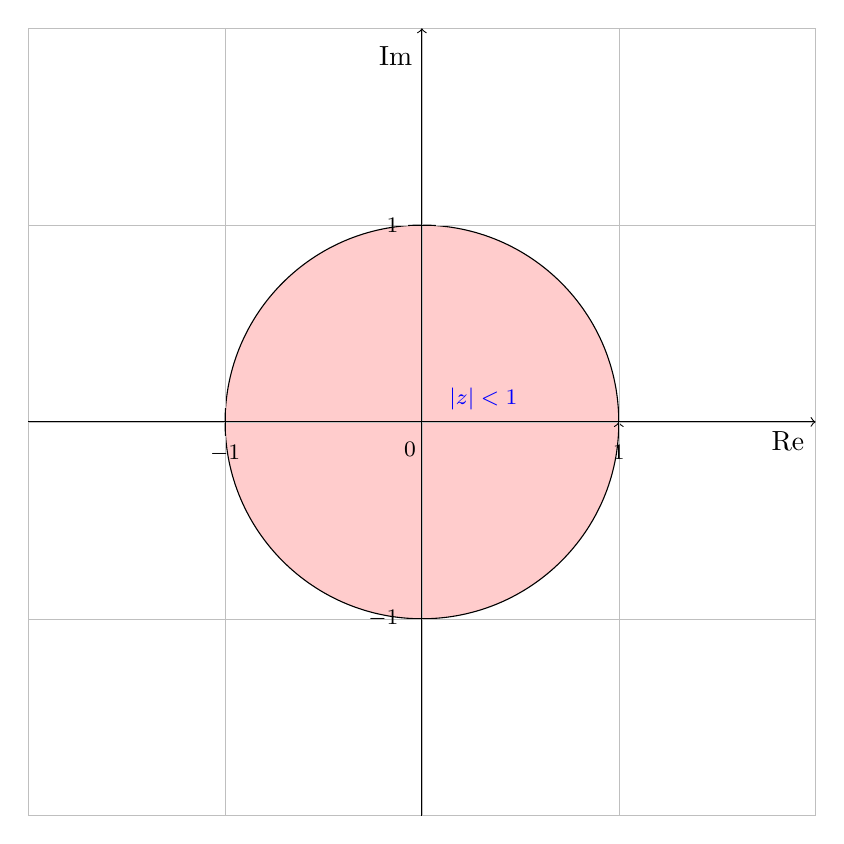
\begin{tikzpicture}[scale=2.5]
			\filldraw [->,draw=black,fill=red!20] (0,0)--(10mm,0mm) arc (0:360:10mm);
			%	\filldraw[->,draw=black,fill=green!20] (0,0) -- (7mm,0mm) arc (0:45:7mm); 
			%	\filldraw[->,fill=orange!20,draw=black,rotate=-45] (0,0) -- (8mm,0mm) arc (0:45:8mm); 
			
			% Gitternetzlinien
			\draw[xstep=1cm, ystep=1cm, very thin, color=lightgray] (-2,-2) grid (2,2);
			% x-Achse
			\draw[->] (-2,0) -- (2,0) node[below,xshift=-1em] {$\mathrm{\mathrm{Re}}$}; 
			%Zahlen auf x-Achse
			\foreach \x in {-1,...,-1}
			\draw[shift={(\x,0)},color=black] (0pt,2pt) -- (0pt,-2pt) node[below] {\footnotesize $\x$};
			\foreach \x in {1,...,1}
			\draw[shift={(\x,0)},color=black] (0pt,2pt) -- (0pt,-2pt) node[below] {\footnotesize $\x$};
			% y-Achse 
			\draw[->] (0,-2) -- (0,2) node[left,yshift=-1em] {$\mathrm{\mathrm{Im}}$};%node[above left]
			%Zahlen auf y-Achse
			\foreach \y in {-1,...,-1}
			\draw[shift={(0,\y)},color=black] (2pt,0pt) -- (-2pt,0pt) node[left] {\footnotesize $\y$};
			\foreach \y in {1,...,1}
			\draw[shift={(0,\y)},color=black] (2pt,0pt) -- (-2pt,0pt) node[left] {\footnotesize $\y$};
			%Ursprung
			\draw[color=black] (-4pt,-4pt) node[right] {\footnotesize $0$};
			
			
			%	\draw [blue,->] (0,0)-.(1,0)node[below,xshift= 0.5em,yshift=1em] {\footnotesize $1+\mathrm{i}$};
			
			%	\draw [blue,->] (0,0)-.(1,-1)node[below,xshift= 0.5em,yshift=1em] {\footnotesize $1-\mathrm{i}$};
			
			\draw [blue] (0.2,0.2) node[xshift= 0.8em,yshift=-0.6em,rotate=0] {\footnotesize $|z|<1$};
			%	\draw [blue] (-0.2,-0.2) node[xshift= 3.8em,yshift=0.1em,rotate=0] {\footnotesize $\overset{\AC}{\alpha}=\frac{\pi}{4}$};
			%	\draw [blue] (-0.6,0.6) node[xshift= 1.3em,yshift=-0.9em,rotate=0] {\footnotesize $\beta=2\pi-\overset{\AC}{\alpha}$};
			
		\end{tikzpicture}\\
		Für alle Punkte innerhalb des Kreises konvergiert diese Reihe.
	\end{center}
\end{quote}
$\bullet$ Für $  z\in\mathbb{R} $ gilt:\\
\begin{quote}
	\begin{align*}
		&f:\{z\in\mathbb{R}\;|\;|z|<1=\;]-1,1[ \;\}\longmapsto\mathbb{R}\\
		&z\longmapsto\sum\limits_{k=0}^{\infty}z^k=\frac{1}{1-z}
	\end{align*}
	Für alle Zahlen im Intervall: $ ]-1,1[ $ konvergiert diese Reihe.\\
	\renewcommand{\baselinestretch}{2.0}\normalsize
	
	\begin{tikzpicture}
		\node at (2,1) [rotate=0,color=black] {$]$};
		\node at (2,0.5) [rotate=0, color=black] {$-1$};
		\draw[->] (0,1) -- (6,1) node [below]{$\mathbb{R}$};
		\draw  (2,1) -- (4,1)[ color=red] ;
		\node at (4,1) [rotate=0,color=black] {$[$};
		\node at (4,0.5) [rotate=0, color=black] {$1$};
	\end{tikzpicture}\ \\
\end{quote}
\renewcommand{\baselinestretch}{1.0}\normalsize
Bemerkung:\\
Die Potenzreihe ist eine Reihe mit konstanten Wert. Konvergiert diese Reihe dann ist sie auch eine Funktion.\\
Im komplexen Bereich konvergiert die Reihe innerhalb eines Kreises (2-Dimensional) und im reellen Bereich in einem 1-Dimensonalen Kreis.\\

\subsection{Konvergenz von Potenzreihen}
\href{https://youtu.be/dGwysWKpoE0}{Video 02}\\
Betrachte folgende Reihe:\\
\begin{align*}
	\sum\limits_{k=0}^{\infty}a_k(z-z_0)^k
\end{align*}
Für welche $ z\in \mathbb{C} $($ z\in\mathbb{R} $) ist die Potenzreihe konvergent?\\
Def.:\\
\begin{align*}
	\sum\limits_{k=0}^{\infty}\underbrace {a_k(z-z_0)^k}_{b_k}
\end{align*}
Wann ist $\sum\limits_{k=0}^{\infty}b_k  $ konvergent?\\
Nach dem Quotientenkriterium gilt:\\
\begin{align*}
	\lim\limits_ {k\to\infty}\bigg|\frac{b_{k+1}}{b_k}\bigg|<1\Rightarrow\;\;\text{Konvergenz }
\end{align*}
Für welche $ z $ gilt dies?\\
\begin{align*}
	\lim\limits_{k\to\infty}\bigg|\frac{b_{k+1}}{b_k}\bigg|=\lim\limits_{k\to\infty}\bigg|\frac{a_{k+1}(z-z_0)^{k+1}}{a_k(z-z_0)^k}\bigg|=\bigg|\frac{a_{k+1}}{a_k}\bigg|\big|z-z_0\big|<1
\end{align*}
Es gilt:\\
Für $ <1 $ konvergent.\\
Für $ >1 $ divergent.\\
Wenn kein Grenzwert existiert und wenn der Grenzwert gegen 1 geht, dann kann man keine Aussage treffen!\\
Nennt man nun $ \lim\limits_ {k\to\infty}\bigg|\frac{b_{k+1}}{b_k}\bigg|=\mathrm{A} $
Dann gilt:\\
\begin{align*}
	\lim\limits_ {k\to\infty}\bigg|\frac{b_{k+1}}{b_k}\bigg|=\mathrm{A}(z-z_0)<1
\end{align*}
\underline{1.Fall:}\\
\begin{quote}
	\begin{align*}
		\mathrm{A}|z-z_0|<1\Leftrightarrow |z-z_0|<\frac{1}{\mathrm{A}}
	\end{align*}
	Die Potenzreihe konvergiert.\\
\end{quote}
\underline{2.Fall:}\\
\begin{quote}
	\begin{align*}
		\mathrm{A}|z-z_0|>1\Leftrightarrow |z-z_0|>\frac{1}{\mathrm{A}}
	\end{align*}
	Die Potenzreihe konvergiert nicht.\\
\end{quote}
\underline{Spezielle Fälle:}\\
\begin{quote}
	$\bullet  \;\; \mathrm{A}=1 $ oder kein Grenzwert.\\
	\begin{quote}
		Kann keine Aussage getroffen werden.
	\end{quote}
	$\bullet  \;\; \mathrm{A}=\infty $ wird zugelassen.\\
	\begin{quote}
		\begin{align*}
			|z-z_0|<\frac{1}{\underbrace {\mathrm{A}}_{\mapsto 0}}
		\end{align*}
		Dies gilt nur, wenn $ z-z_0=0 $ also der Grenzwert wird Null (trivial). Die Reihe konvergiert.\\
	\end{quote}
	$\bullet  \;\; \mathrm{A}=0 $
	\begin{quote}
		\begin{align*}
			\mathrm{A}|z-z_0|=0|z-z_0|<1
		\end{align*}
		Potenzreihe konvergiert für alle $ z $.\\
	\end{quote}
\end{quote}
Die Potenzreihe:\\
\begin{align*}
	\sum\limits_{k=0}^{\infty}a_k(z-z_0)^k
\end{align*}
konvergiert für alle $ |z-z_0| $, wenn gilt:\\
\begin{align*}
	|z-z_0|<R
\end{align*}
wobei für $ R $ gilt:\\
\begin{align*}
	R:=\frac{1}{\lim\limits_ {k\to\infty}\bigg|\frac{a_{k+1}}{a_k}\bigg|}
\end{align*}
\newpage
\noindent
Bemerkung:\\
$ |z-z_0|<R\;\;z\in \mathbb{C} $ ist ein Kreis von Radius $ R $ um $ z_0 $\\
\begin{center}
	
	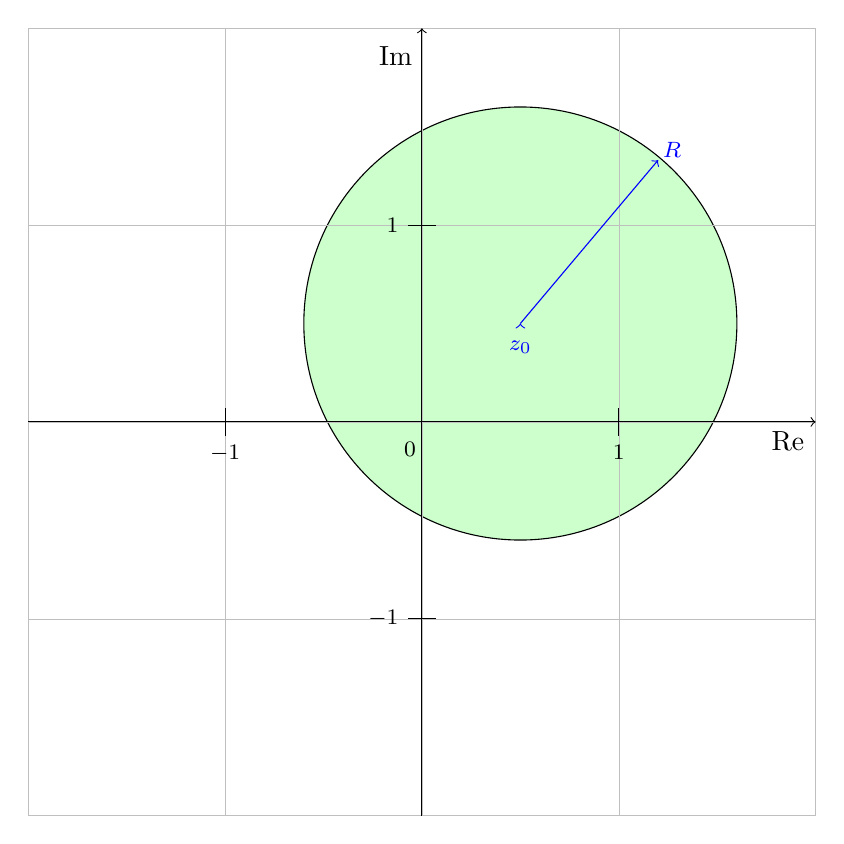
\begin{tikzpicture}[scale=2.5]
		%\filldraw [->,draw=black,fill=red!20] (0,0)--(12mm,0mm) arc (0:360:12mm);
		%	\filldraw[->,draw=black,fill=green!20] (0,0) -- (7mm,0mm) arc (0:45:7mm); 
		%	\filldraw[->,fill=orange!20,draw=black,rotate=-45] (0,0) -- (8mm,0mm) arc (0:45:8mm); 
		\filldraw [->,draw=black,fill=green!20](0.5,0.5) circle (11mm);
		% Gitternetzlinien
		\draw[xstep=1cm, ystep=1cm, very thin, color=lightgray] (-2,-2) grid (2,2);
		% x-Achse
		\draw[->] (-2,0) -- (2,0) node[below,xshift=-1em] {$\mathrm{\mathrm{Re}}$}; 
		%Zahlen auf x-Achse
		\foreach \x in {-1,...,-1}
		\draw[shift={(\x,0)},color=black] (0pt,2pt) -- (0pt,-2pt) node[below] {\footnotesize $\x$};
		\foreach \x in {1,...,1}
		\draw[shift={(\x,0)},color=black] (0pt,2pt) -- (0pt,-2pt) node[below] {\footnotesize $\x$};
		% y-Achse 
		\draw[->] (0,-2) -- (0,2) node[left,yshift=-1em] {$\mathrm{\mathrm{Im}}$};%node[above left]
		%Zahlen auf y-Achse
		\foreach \y in {-1,...,-1}
		\draw[shift={(0,\y)},color=black] (2pt,0pt) -- (-2pt,0pt) node[left] {\footnotesize $\y$};
		\foreach \y in {1,...,1}
		\draw[shift={(0,\y)},color=black] (2pt,0pt) -- (-2pt,0pt) node[left] {\footnotesize $\y$};
		%Ursprung
		\draw[color=black] (-4pt,-4pt) node[right] {\footnotesize $0$};
		
		
		%	\draw [blue,->] (0,0)-.(1,0)node[below,xshift= 0.5em,yshift=1em] {\footnotesize $1+\mathrm{i}$};
		
		%	\draw [blue,->] (0,0)-.(1,-1)node[below,xshift= 0.5em,yshift=1em] {\footnotesize $1-\mathrm{i}$};
		\draw[blue,->](5mm,5mm) node[xshift= 0,yshift=-3mm,rotate=0] {\footnotesize $z_0$};
		\draw[blue,->] (0.5,0.5)--(12mm,13.3mm)node[below,xshift= 0.5em,yshift=1em] {\footnotesize $R$};
		
		%	\draw [blue] (-0.2,-0.2) node[xshift= 3.8em,yshift=0.1em,rotate=0] {\footnotesize $\overset{\AC}{\alpha}=\frac{\pi}{4}$};
		%	\draw [blue] (-0.6,0.6) node[xshift= 1.3em,yshift=-0.9em,rotate=0] {\footnotesize $\beta=2\pi-\overset{\AC}{\alpha}$};
		
	\end{tikzpicture}\\
\end{center}
$ |z-z_0|<\mathrm{R}\;\;z\in \mathbb{R} $ ist eine Gerade mit Abstand $ R $ um $ z_0 $\\
\begin{center}
	Für $ z_0=2$ gilt:\\ 
	
	\begin{tikzpicture}
		\node at (5,1) [rotate=0,color=black] {$|$};
		\node at (2,1) [rotate=0,color=black] {$]$};
		\node at (2,0.5) [rotate=0, color=black] {$2-\mathrm{R}$};
		\draw[->] (0,1) -- (10,1) node [below]{$\mathbb{R}$};
		\draw  (2,1) -- (8,1)[ color=red] ;
		\node at (8,1) [rotate=0,color=black] {$[$};
		\node at (8,0.5) [rotate=0, color=black] {$2+\mathrm{R}$};
		\node at (5,0.5) [rotate=0, color=black] {$2$};
	\end{tikzpicture}\ \\
\end{center}
\subsubsection{ Aufgabe 1 zur Konvergenz von Potenzreihen}
\href{https://youtu.be/PZkcdZNx7I4}{Video 03}\\
Bestimme den Konvergenzradius von:\\
\begin{align*}
	\sum\limits_{k=0}^{\infty}\frac{\mathrm{e}^{2k}\cdot x^k}{k+1}
\end{align*}
Zur Berechnung des Konvergenzradius formt man entsprechend um:\\
\begin{align*}
	\sum\limits_{k=0}^{\infty}\frac{\mathrm{e}^{2k}\cdot x^k}{k+1}=\sum\limits_{k=0}^{\infty}\underbrace {\frac{\mathrm{e}^{2k}}{k+1}}_{a_k}(x-0)^k
\end{align*}
Es gilt mit $ a_k=\frac{\mathrm{e}^{2k}}{k+1} $:\\
\begin{align*}
	\mathrm{R}=\frac{1}{\lim\limits_ {k\to\infty}\big|\frac{a_{k+1}}{a_k}\big|}
\end{align*}
Nun den Grenzwert berechen:\\
\begin{align*}
	\lim\limits_ {k\to\infty}\bigg|\frac{a_{k+1}}{a_k}\bigg|=\lim\limits_ {k\to\infty}\bigg|\frac{\mathrm{e}^{2(k+1)}(k+1)}{(k+2)\mathrm{e}^{2k}}\bigg|=\lim\limits_ {k\to\infty}\mathrm{e}^2\;\;\frac{k+1}{k+2}=\mathrm{e}^2\lim\limits_ {k\to\infty}\frac{k\big(\frac{1}{k}+1\big)}{k\big(\frac{2}{k}+1\big)}=\mathrm{e}^2
\end{align*}
Für den Konvergenzradius gilt:\\
\begin{align*}
	\mathrm{R}=\frac{1}{\lim\limits_ {k\to\infty}\big|\frac{a_{k+1}}{a_k}\big|}=\frac{1}{\mathrm{e}^2}
\end{align*}
Fazit:\\
\begin{align*}
	\mathrm{R}=\frac{1}{\mathrm{e}^2}
\end{align*}
Für $ |x-\underbrace {x_0}_{x_0=0}|=|x|<\frac{1}{\mathrm{e}^2} $ ist die Reihe:$\sum\limits_{k=0}^{\infty}\frac{\mathrm{e}^{2k}\cdot x^k}{k+1}  $ konvergent und definiert dort eine Funktion.\\
\\
Für die Randpunkte muss man noch die Konvergenz untersuchen.\\
Es gilt:\\
\begin{align*}
	|x|<\frac{1}{\mathrm{e}^2}\Rightarrow x_1=\frac{1}{\mathrm{e}^2},\; x_2=-\frac{1}{\mathrm{e}^2}
\end{align*}
\textbullet\;\; Für$\;\;x_1=\frac{1}{\mathrm{e}^2} $ gilt:\\
\begin{align*}
	\sum\limits_{k=0}^{\infty}\frac{\mathrm{e}^{2k}\cdot \big(\frac{1}{\mathrm{e}^2}\big)^k}{k+1}=\sum\limits_{k=0}^{\infty}\frac{\mathrm{e}^{2k}}{k+1}\bigg(\frac{1}{\mathrm{e}^2}\bigg)^k=\sum\limits_{k=0}^{\infty}\frac{\mathrm{e}^{2k}}{(k+1)\mathrm{e}^{2k}}=\sum\limits_{k=0}^{\infty}\frac{1}{k+1}\Rightarrow\text{divergent (Harmonische Reihe) }
\end{align*}
\textbullet\;\; Für$\;\;x_1=-\frac{1}{\mathrm{e}^2} $ gilt:\\
\begin{align*}
	\sum\limits_{k=0}^{\infty}\frac{\mathrm{e}^{2k}}{k+1}\bigg(\frac{-1}{\mathrm{e}^2}\bigg)^k&=\sum\limits_{k=0}^{\infty}\frac{\mathrm{e}^{2k}}{k+1}(-1)^k\bigg(\frac{1}{\mathrm{e}^2}\bigg)^k=\sum\limits_{k=0}^{\infty}\frac{\mathrm{e}^{2k}}{k+1}(-1)^k\bigg(\frac{1}{\mathrm{e}^{2k}}\bigg)\\&=\sum\limits_{k=0}^{\infty}(-1)^k\frac{1}{k+1}\Rightarrow\text{konvergent (Leibnizkritrium) }
\end{align*}
Fazit:\\
Die Reihe $ \sum\limits_{k=0}^{\infty}\frac{\mathrm{e}^{2k}\cdot x^k}{k+1} $ ist konvergent im Bereich von: $ x\in\big[-\frac{1}{\mathrm{e}^2},\frac{1}{\mathrm{e}^2}\big[\; $.\\
\newpage
\noindent
\subsubsection{ Aufgabe 2 zur Konvergenz von Potenzreihen}
\href{https://youtu.be/8TeaUxqFeuk}{Video 04}\\
Bestimme den Konvergenzradius von:\\
\begin{align*}
	\sum\limits_{k=1}^{\infty}\frac{(4z-2)^k}{k^4}\;\;\text{für}\;\;z\in \mathbb{C}
\end{align*}
Zum Konvergenzradius:\\
\begin{align*}
	\sum\limits_{k=1}^{\infty}\frac{(4z-2)^k}{k^4}=\sum\limits_{k=1}^{\infty}\frac{(4(z-\frac{1}{2}))^k}{k^4}=\sum\limits_{k=0}^{\infty}\underbrace {\frac{4^k}{k^4}}_{=a_k}\bigg(z-\frac{1}{2}\bigg)^k
\end{align*}
Es gilt mit $ a_k=\frac{4^k}{k^4} $:
\begin{align*}
	\mathrm{R}=\frac{1}{\lim\limits_ {k\to\infty}\big|\frac{a_{k+1}}{a_k}\big|}
\end{align*}
Nun den Grenzwert berechnen:\\
\begin{align*}
	\lim\limits_ {k\to\infty}\bigg|\frac{a_{k+1}}{a_k}\bigg|=\lim\limits_ {k\to\infty}\frac{4^{k+1}}{(k+1)^4}\frac{k^4}{4^k}=\lim\limits_ {k\to\infty}4\bigg(\frac{k}{k+1}\bigg)^4=\lim\limits_ {k\to\infty}4\bigg(\underbrace {\frac{k}{k(1+\frac{1}{k})}}_{=1}\bigg)=4
\end{align*}
Folglich ist der Konvergenzradius von: $\sum\limits_{k=1}^{\infty}\frac{(4z-2)^k}{k^4}  $:\\
\begin{align*}
	\mathrm{R}&=\frac{1}{\lim\limits_ {k\to\infty}\big|\frac{a_{k+1}}{a_k}\big|}=\frac{1}{4}\\
	\mathrm{R}&=\frac{1}{4}
\end{align*}
\newpage
\noindent
\subsection{Differentiation von Potenzreihen }
\href{https://youtu.be/kpaMK4KSYDg}{Video 05}\\
\begin{center}
	
	
	\fbox{\parbox  {155mm} {
			Sei $\sum\limits_{k=0}^{\infty}a_k(x-x_0)^k  $ eine reelle Potenzreihe mit Konvergenzradius: $ \mathrm{R}>0$.\\ Dann ist: 
			\begin{align*}
				f:\; ]x_o-\mathrm{R} , x_0+\mathrm{R}[\; \longmapsto \mathbb{R}\;\; \text{mit } f(x)=\sum\limits_{k=0}^{\infty}a_k(x-x_0)^k
			\end{align*}\\
			eine differenzierbare Funktion mit: 
			\begin{align*}
				f'(x)=\sum\limits_{k=0}^{\infty}\big(a_k(x-x_0)^k\big)'
	\end{align*}}}
\end{center}
Bemerkung:\\
Wie schon bekannt ist eine Potenzreihe mit $ \mathrm{R}>0 $ zwischen $ ]x_o-\mathrm{R} , x_0+\mathrm{R}[  $ eine Funktion und deshalb auch differenzierbar.\\
\\
Für einen Term gilt:\\
\begin{align*}
	\big(a_k(x-x_0)^k\big)'=a_k\cdot k(x-x_0)^{k-1}\\
\end{align*}
Dann gilt für die Reihe:\\
\begin{align*}
	\sum\limits_{k=0}^{\infty}\big(a_k(x-x_0)^k\big)'=\sum\limits_{k=0}^{\infty}a_k\cdot k(x-x_0)^{k-1}
\end{align*}
Für $ k=0 $ gilt:\\
\begin{align*}
	a_0\cdot 0(x-x_0)^{0-1}=0
\end{align*}
Dann gilt:\\
\begin{align*}
	\sum\limits_{k=1}^{\infty}a_k\cdot k(x-x_0)^{k-1}
\end{align*}
Mit Indexverschiebung ergibt sich:\\
\begin{align*}
	\sum\limits_{k=0}^{\infty}a_{k+1}(k+1)(x-x_0)^{k}
\end{align*}
Für die Potenzreihe mit dem Konvergenzradius: $ \mathrm{R}>0 $ gilt dann:\\
\begin{align*}
	\sum\limits_{k=0}^{\infty}\big(a_k(x-x_0)^k\big)'=\sum\limits_{k=0}^{\infty}a_{k+1}(k+1)(x-x_0)^{k}
\end{align*}
Beispiel:\\
Wir betrachten:\\
\begin{align*}
	\sum\limits_{k=0}^{\infty} x^k\;\;\text{mit Konvergenzradius }\mathrm{R}=1
\end{align*}
Es gilt für:\\
\begin{align*}
	|x|<1 : f(x)=\sum\limits_{k=0}^{\infty}x^k=\frac{1}{1-x}
\end{align*}
Die Funktion $ f(x) $ ist differenzierbar dann gilt:\\
\begin{align*}
	f'(x)&=\sum\limits_{k=0}^{\infty}\big(a_k(x-x_0)^k\big)'=\sum\limits_{k=0}^{\infty}a_{k+1}(k+1)(x-x_0)^{k}\\
	a_k&=1\\
	x_0&=0\\
&=\sum\limits_{k=0}^{\infty}\big(1\cdot(x-0)^k\big)'=\sum\limits_{k=0}^{\infty}1\cdot(k+1)(x-0)^k\\
	f'(x)	&=\sum\limits_{k=0}^{\infty}(k+1)(x)^k\\
\end{align*}
Für $ f'(x)=\big(\frac{1}{1-x}\big)' $ gilt:\\
\begin{align*}
	f'(x)=\bigg(\frac{1}{1-x}\bigg)'=\bigg((1-x)^{-1}\bigg)'=-1\cdot(1-x)^{-2}(-1)=\frac{1}{(1-x)^2}
\end{align*}
Fazit:\\
\begin{align*}
	\sum\limits_{k=0}^{\infty}(k+1)x^k=\frac{1}{(1-x)^2}\;\;\text{und hat Konvergenzradius: }\mathrm{R}=1
\end{align*}
\newpage
\noindent
\subsection{Integration von Potenzreihen}
\href{https://youtu.be/0rKwoivWboE}{Video 06}\\
\begin{center}
	
	
	\fbox{\parbox  {155mm} {
			Sei $\sum\limits_{k=0}^{\infty}a_k(x-x_0)^k  $ eine reelle Potenzreihe mit Konvergenzradius: $ \mathrm{R}>0$.\\ Dann ist: 
			\begin{align*}
				f:\; ]x_o-\mathrm{R} , x_0+\mathrm{R}[\; \longmapsto \mathbb{R}\;\; \text{mit } f(x)=\sum\limits_{k=0}^{\infty}a_k(x-x_0)^k
			\end{align*}\\
			eine integrierbare Funktion mit:
			\begin{align*}
				\int\limits_{}^{}f(x) \mathrm{d}x=\sum\limits_{k=0}^{\infty}\int\limits_{}^{} a_k(x-x_0)^k dx
			\end{align*}	
	}}
\end{center}
Es gilt für die Potenzreihe:\\
\begin{align*}
	\int\limits_{}^{} a_x(x-x_0)^k \mathrm{d}x=a_k\cdot \frac{(x-x_0)^{k+1}}{k+1}+\alpha_k\;\;\text{mit }\alpha_k\in\mathbb{R}
\end{align*}
Dies ergibt eine neue Potenzreihe mit dem gleichen Konvergenzradius: $ \mathrm{R}=1 $\\
\\
Beispiel:\\
Betrachte:\\
\begin{align*}
	f(x)=\sum\limits_{k=0}^{\infty}x^k\;\;\text{mit }\;\;|x|<1\;\;\mathrm{R}=1
\end{align*}
Für das Integral gilt:\\
\begin{align*}
	\int\limits_{}^{}f(x) \mathrm{d}x=\sum\limits_{k=0}^{\infty}\int\limits_{}^{} x^k dx=\sum\limits_{}^{}\frac{x^{k+1}}{k+1}+\alpha\;\;\text{mit }\alpha\in\mathbb{R}
\end{align*}
Nun gilt auch:\\
\begin{align*}
	&\sum\limits_{k=0}^{\infty}x^k=\frac{1}{1-x}\\
	&\Rightarrow \int\limits_{}^{} \frac{1}{1-x} \mathrm{d}x=-\ln(1-x)+\alpha,\;\;\text{mit } \alpha\in\mathbb{R}
\end{align*}
Fazit:\\
\begin{align*}
	\sum\limits_{k=0}^{\infty}\frac{x^{k+1}}{k+1}=-\ln(1-x)=\ln\bigg(\frac{1}{1-x}\bigg)
\end{align*}
Bemerkung:\\
\begin{align*}
	-\ln(a)=\ln(a^{-1})=\ln\bigg(\frac{1}{a}\bigg)
\end{align*}
Durch die Integation kommt man zu einer neuen Potenzreihe mit dem gleichen Konvergenzradius $ \mathrm{R}=1 $ wie bei der Funktion: $ f(x)=\sum\limits_{k=0}^{\infty}x^k $.
\subsection{Die Taylorreihe}
\href{https://youtu.be/lnDbJwbBlqY}{Video 07}\\
\begin{center}
	\underline{Taylorreihe}	
\end{center}
Sei $ f:\mathbb{R}\supset \mathbb{I}\rightarrow\mathbb{R}\;\; n$-mal differenzierbar (im Intervall $  \mathbb{I} $) dann \\
gilt mit $ x_0\in \mathbb{I} $:\\
\begin{align*}
	f(x)=\sum\limits_{k=0}^{n}\frac{f^k (x_0)}{k!}(x-x_0)^k+\mathrm{R}_n(x)
\end{align*}
Wobei der Grenzwert vom Rest gegen Null geht für:\\
\begin{align*}
	\lim\limits_ {x\to x_0}\frac{\mathrm{R}_n (x)}{(x-x_0)^k}=0
\end{align*}
Wenn die Funktion beliebig oft differenzierbar ist, dann gilt für den Rest:\\
\begin{align*}
	\lim\limits_ {n\to\infty}\mathrm{R}_n (x)=0
\end{align*}
Daraus folgt dann, dass man die Funktion auch als Potenzreihe schreiben kann, weil der Rest Null wird.\\
\begin{align*}
	f(x)=\sum\limits_{k=0}^{\infty}a_k(x-x_0)^k=\sum\limits_{k=0}^{\infty}\frac{f^k (x_0)}{k!}(x-x_0)^k
\end{align*}
\subsubsection{Beispiel zur Taylorreihe}
\href{https://youtu.be/AJxupcdeQJc}{Video 08}\\
Beispiel:\\
Betrachten wir eine beliebig oft differnzierbare Funktion:\\
\begin{align*}
	f(x)=\mathrm{e}^x\;\;\text{und  } x_0=0
\end{align*}
Es gilt:\\
\begin{align*}
	&f^k (x)=\mathrm{e}^x\\
	&f^k (x_0)=\mathrm{e}^0=1
\end{align*}
Die Taylorreihe lautet dann:\\
\begin{align*}
	f(x)=\sum\limits_{k=0}^{n}\frac{1}{k!}(x-x_0)^k+\mathrm{R}_n(x)=\frac{x^k}{k!}+\mathrm{R}_n(x)
\end{align*}
\underline{Lagrange'sche Restglieddarstellung:}
\begin{align*}
	\mathrm{R}_n(x)&=\frac{f^{k+1}(a)}{(n+1)!}\cdot x^{n+1}\;\;\text{mit $ a $ zwischen $ x $ und $ x_0 $}\\
	&=\frac{\mathrm{e}^{a}}{(n+1)!}\cdot x^{n+1}
\end{align*}
Betrachte:\\
\begin{align*}
	\lim\limits_ {n\to\infty}f(x)&=\lim\limits_ {n\to\infty}\mathrm{e}^{a}\frac{x^{n+1}}{(n+1)!}=\mathrm{e}^{a}\lim\limits_ {n\to\infty}\frac{x^{n+1}}{(n+1)!}\\
	&=\mathrm{e}^{a}\lim\limits_ {n\to\infty}\frac{x\cdot x\cdot x\cdot\dots}{1\cdot 2 \cdot 3\dots  n (n+1)}\\
	&=\mathrm{e}^{a}\bigg(\lim\limits_ {n\to\infty}\bigg(\frac{x}{1}\bigg)\cdot \lim\limits_ {n\to\infty}\bigg(\frac{x}{2}\bigg)\cdot \lim\limits_ {n\to\infty}\bigg(\frac{x}{3}\bigg)\dots \underbrace {\lim\limits_ {n\to\infty}\bigg(\frac{x}{n}\bigg)}_{=0}\cdot \underbrace {\lim\limits_ {n\to\infty}\bigg(\frac{x}{n+1}\bigg)}_{=0}\bigg)=0
\end{align*}
Fazit:\\
Mit $ f(x)=\mathrm{e}^x $ und $ x_0=0 $ ergibt sich als Taylorreihe:\\
\begin{align*}
	\mathrm{e}^x=f(x)=\sum\limits_{k=0}^{\infty}\frac{1}{k!}(x-x_0)^k=\sum\limits_{k=0}^{\infty}\frac{1}{k!}x^k
\end{align*}
\underline{Bestimmung des Konvergenzradius:}\\
\begin{align*}
	\mathrm{R}=\frac{1}{\lim\limits_ {k\to\infty}\big|\frac{a_{k+1}}{a_k}\big|}
\end{align*}
Es gilt:\\
\begin{align*}
	a_k=\frac{1}{k!}
\end{align*}
\begin{align*}
	\bigg|\frac{a_{k+1}}{a_k}\bigg|=\frac{\frac{1}{(k+1)!}}{\frac{1}{k!}}=\frac{k!}{(k+1)!}
\end{align*}
Für den Grenzwert gilt dann:\\
\begin{align*}
	\lim\limits_ {k\to\infty}\frac{k!}{(k+1)!}=\lim\limits_ {k\to\infty}\frac{1\cdot 2\cdot 3\dots k}{1\cdot 2\cdot 3\dots k(k+1)}=\lim\limits_ {k\to\infty}\frac{1}{k+1}=0\\
\end{align*}
Der Konvergenzradius ist dann:\\
\begin{align*}
	\mathrm{R}=\frac{1}{\lim\limits_ {k\to\infty}\big|\frac{a_{k+1}}{a_k}\big|}=\frac{1}{\lim\limits_ {k\to\infty}\frac{1}{k+1}}=\infty
\end{align*}
Fazit:\\
Die Taylorreihe von $ \mathrm{e}^x $ konvergiert für alle $ x\in\mathbb{R} $\\

































































